В нашей работе используется тиратрон ТГ3-01/1.3Б, заполненный инертным газом.
Схематическое изображение тиратрона и его конструкция приведены на рис.
(\ref{img::sch_tirat}).
\begin{wrapfigure}{r}{0.4\textwidth}
  \centering
  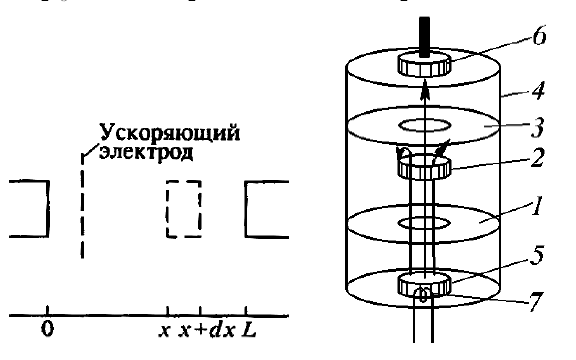
\includegraphics[width=\linewidth]{scheme_tirat.png}
  \caption{{Схема тиратрона (слева) и его конструкция (справа): \\
  1, 2, 3 --- сетки, 4 --- внешний металлический цилиндр, 5 --- катод, \\ 6 ---
  анод, 7 --- накаливаемая спираль}}
  \label{img::sch_tirat}
\end{wrapfigure}
Электроны, эмитируемые катодом тиратрона, ускоряются напряжением $V$,
приложенным между катодом и ближайшей к нему сеткой. Затем электроны
рассеиваются на атомах инертного газа. Все сетки 1, 2, 3 соединены между собой и
имеют одинаковый потенциал, примерно равный потенциалу анода 6. Поэтому между
первой сеткой 1 и анодом практически нет поля. Рассеянные электроны отклоняются
в сторону и уходят на сетку, а оставшаяся часть электронов достигает анода и
создает анодный ток $I_a$. Таким образом, поток электронов $N(x)$ на расстоянии
$x$ от ускоряющей сетки (т.е. число электронов, проходящих через поперечное
сечение лампы в точке $x$ в единицу времени) уменьшается с ростом $x$ от
начального значения $N_0$ у катода (в точке $x = 0$) до некоторого значения
$N_a$ у анода (в точке $x = L$).

Рассмотрим теперь, какова должна быть реальная вольт-амперная характеристика
(ВАХ) тиратрона. Выделим в газе на расстоянии $x$ тонкий слой с площадью
поперечного сечения $S$ и толщиной $dx$. Этот слой содержит $\nu = n_a S dx$
атомов газа ($n_a$ -- концентрация атомов газа в лампе). Суммарная рассеивающая
поверхность этих атомов $\Delta = \mu \Delta_a$, где $\Delta_a$ -- площадь
поперечного сечения атома. Обозначим через $dN$ убыль потока электронов в
результате прохождения слоя $dx$; тогда $dN/N(x)$ есть доля электронов, которые
рассеялись, или вероятность рассеяния в слое. Для рассеяния электрона в слое
необходимо выполнение двух независимых событий -- электрон должен <<наткнуться>>
в слое на атом, и, кроме того, он должен на этом атоме рассеяться.
Следовательно, вероятность $dN/N(x)$ рассеяния электрона в слое равна
произведению двух вероятностей -- вероятности для электрона в слое $dx$
встретить атом газа (она равна $\Delta / S$ -- доли площади поперечного сечения
слоя, перекрываемого атомами) и вероятности рассeяния на атоме $\omega(V)$:

\begin{equation}
  - \frac{dN}{N(x)} = \frac{\Delta}{S} \cdot \omega(V) = n_a \Delta_a \omega(V) dx
\end{equation}

Интегрируя это соотношение от $0$ до $L$ и заменяя поток электронов на ток $I =
Ne$, получаем уравнение ВАХ:

\begin{equation} \label{eq::current}
  I_a = I_0 \e^{ - C \omega(V)}, \: C = L \cdot n_a \Delta_a
\end{equation}

где $I_0 = e N_0$ -- ток катода, $I_a = e N_a$ -- анодный ток.
\begin{wrapfigure}{r}{0.5\textwidth}
  \centering
  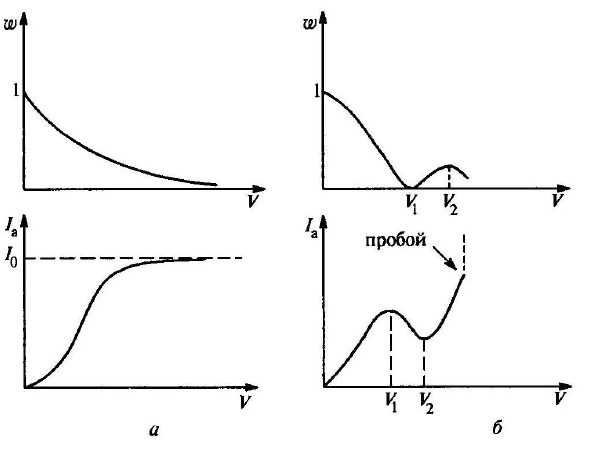
\includegraphics[width=\linewidth]{VAH_tirat.png}
  \caption{ {Вероятность рассeяния электрона атомом инертного газа и ВАХ
    тиратрона при классическом (а) и квантовом (б) рассмотрении.}}
  \label{img::vah_tirat}
\end{wrapfigure}
Согласно классическим представлениям, сечение рассеяния электрона на атоме
должно падать монотонно с ростом $V$ (обратно пропорционально скорости
электрона, т.е. обратно пропорционально корню квадратному из его энергии), а
значит ВАХ будет монотонна возрастающей функцией, как это показано на рис.
(\ref{img::vah_tirat}а). По квантовым соображения вероятность рассеяния
электронов и соответствующая ВАХ должны иметь вид, показанный на рис.
(\ref{img::vah_tirat}б).

Согласно формуле \eqref{eq::current}, по измеренной ВАХ тиратрона можно
определить зависимость вероятности рассеяния электрона от его энергии из
соотношения

\begin{equation}\label{eq::probability}
  \omega(V) = -\frac{1}{C} \cdot \ln \frac{I_a(V)}{I_0}
\end{equation}

\newpage
\begin{wrapfigure}{r}{0.4\textwidth}
  \centering
  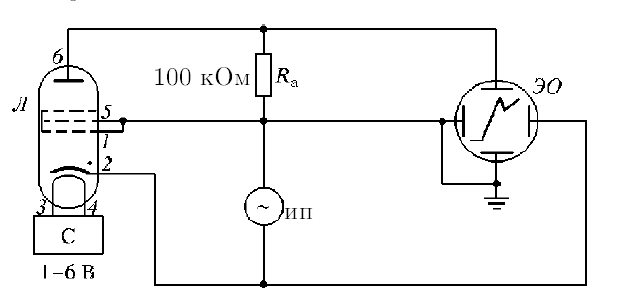
\includegraphics[width=\linewidth]{ON_tirat.png}
  \caption{ {Схема включения тиратрона}}
  \label{img::on_tirat}
\end{wrapfigure}
Принципиальная схема установки для изучения эффекта Рамзауэра приведена на рис.
(\ref{img::on_tirat}). На лампу подается синусоидальное напряжение частоты $50$
Гц от источника питания, $C$ -- стабилизированный блок накала катода;
исследуемый сигнал подается на электронный осциллограф; цифрами обозначены
номера ножек лампы.

Реально на экране осциллографа удается надежно наблюдать лиш один(первый, при $n
= 1$) минимум в сечении рассеяния электронов и следующий за ним максимум. Дело в
том, что уже при $n = 2$ напряженность поля столь велика, что с большой
вероятностью происходить ионизация атомов и возникает пробой тиратрона. Кроме
того, как показывает расчет, с ростом $n$ глубина минимума резко уменьшается,
что приводит к не столь ярко выраженному эффекту <<просветления>> газа.

Схема экспериментальной установки, изображенная на рис. (\ref{img::on_tirat}) в
нашей работе конструктивно осуществлена следующим образом. Лампа-тиратрон
ТГЗ-01/1.3Б, заполненная инертным газом, расположена непосредственно на корпусе
блока источника питания (БИП). Напряжение к электродам лампы подается от
источников питания, находящихся в корпусе прибора. Регулировка напряжения и
выбор режима работы установки производится при помощи ручек управления,
выведенных на лицевую панель БИП (рис. (\ref{img::whole_tirat})).

\begin{figure}[h!]
  \centering
  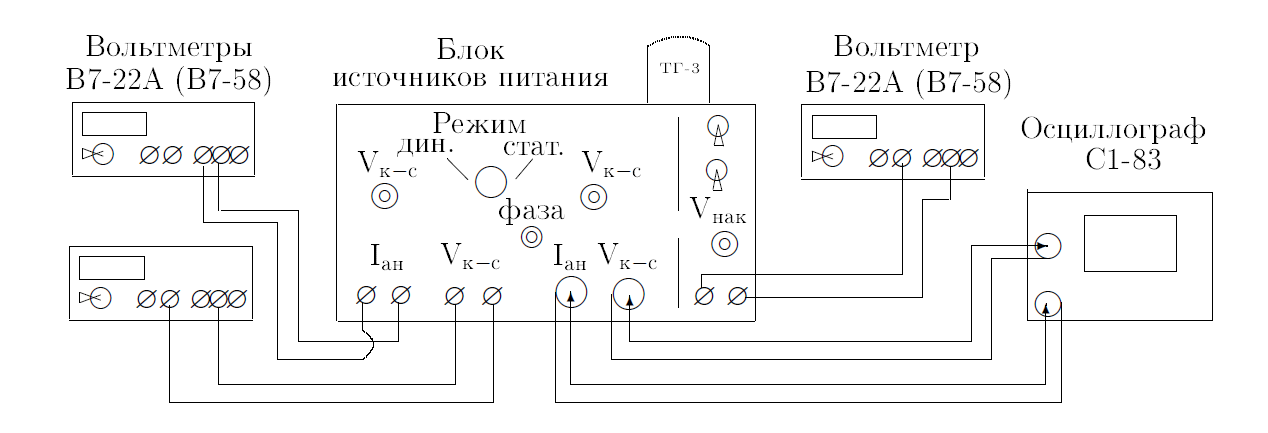
\includegraphics[width=\linewidth]{whole_scheme_tirat.png}
  \caption{ {Блок-схема экспериментальной установки}}
  \label{img::whole_tirat}
\end{figure}
